% Chapter Template

\chapter{Introduction} % Main chapter title

\label{Chapter 1} % Change X to a consecutive number; for referencing this chapter elsewhere, use \ref{ChapterX}

\lhead{Chapter 1. \emph{Introduction}} % Change X to a consecutive number; this is for the header on each page - perhaps a shortened title

%----------------------------------------------------------------------------------------
%	SECTION 1
%---------------------------------------------------------------------------------------
Synthetic aperture radar (SAR) can provide more useful information of targets than the optical data from traditional remote sensing. Therefore, the SAR data has been used for various remote sensing applications such as land cover classification, urban extraction, and analysis. Remote sensing has provided invaluable information to forestry. Remote sensing images can be used to map the spatial extent of forest resources. We are interested in the detection of forest cover in an area when provided with its corresponding SAR data.


\section{Motivation}

Forests are a very important natural resource and provides habitats for animals and livelihoods for humans. Forests also offer watershed protection, prevent soil erosion and mitigate climate change. Reliable and timely information on forest area and land use nearby forest is of great importance to planners and policymakers for efficient wildlife and forest conservation and for taking decisions on many other related issues. Optical data have been used for the assessment of mapping forest cover at medium and high resolutions. Nonetheless, the utility of optical data is highly affected by atmospheric conditions. SAR provides an alternative to obtain information. Along with single polarization datasets, dual or fully polarimetric SAR images have been used. The Indian RISAT-1 satellite has provided hybrid polarimetric high resolution data and the data availability has allowed us to evaluate the suitability of hybrid polarimetric data for forest detection and classification. 

\section{Problem Description and Objective}



\paragraph{Literature Survey}

This is a sample. Write about referred papers. Cite like this \cite{c7}. Another example would be this \cite{c1}. More citations like this \cite{c3}.

\paragraph{Research gaps}
Typically include research gaps for your study. 
\paragraph{Objective}
Similarly objectives of study. 
\paragraph{Scope}
Define scope of study. 
\paragraph{An algorithm}
How you could refer to figures: This is an example. (Refer \ref{fig5}). You can add equations like this Eq. (\ref{eq1})
\begin{equation}
\label{eq1}
  SDR = sd(T) - \sum_{i}\frac{{T}_{i}}{|T|}\times sd({T}_{i})
\end{equation}

\begin{figure}[]
\centering
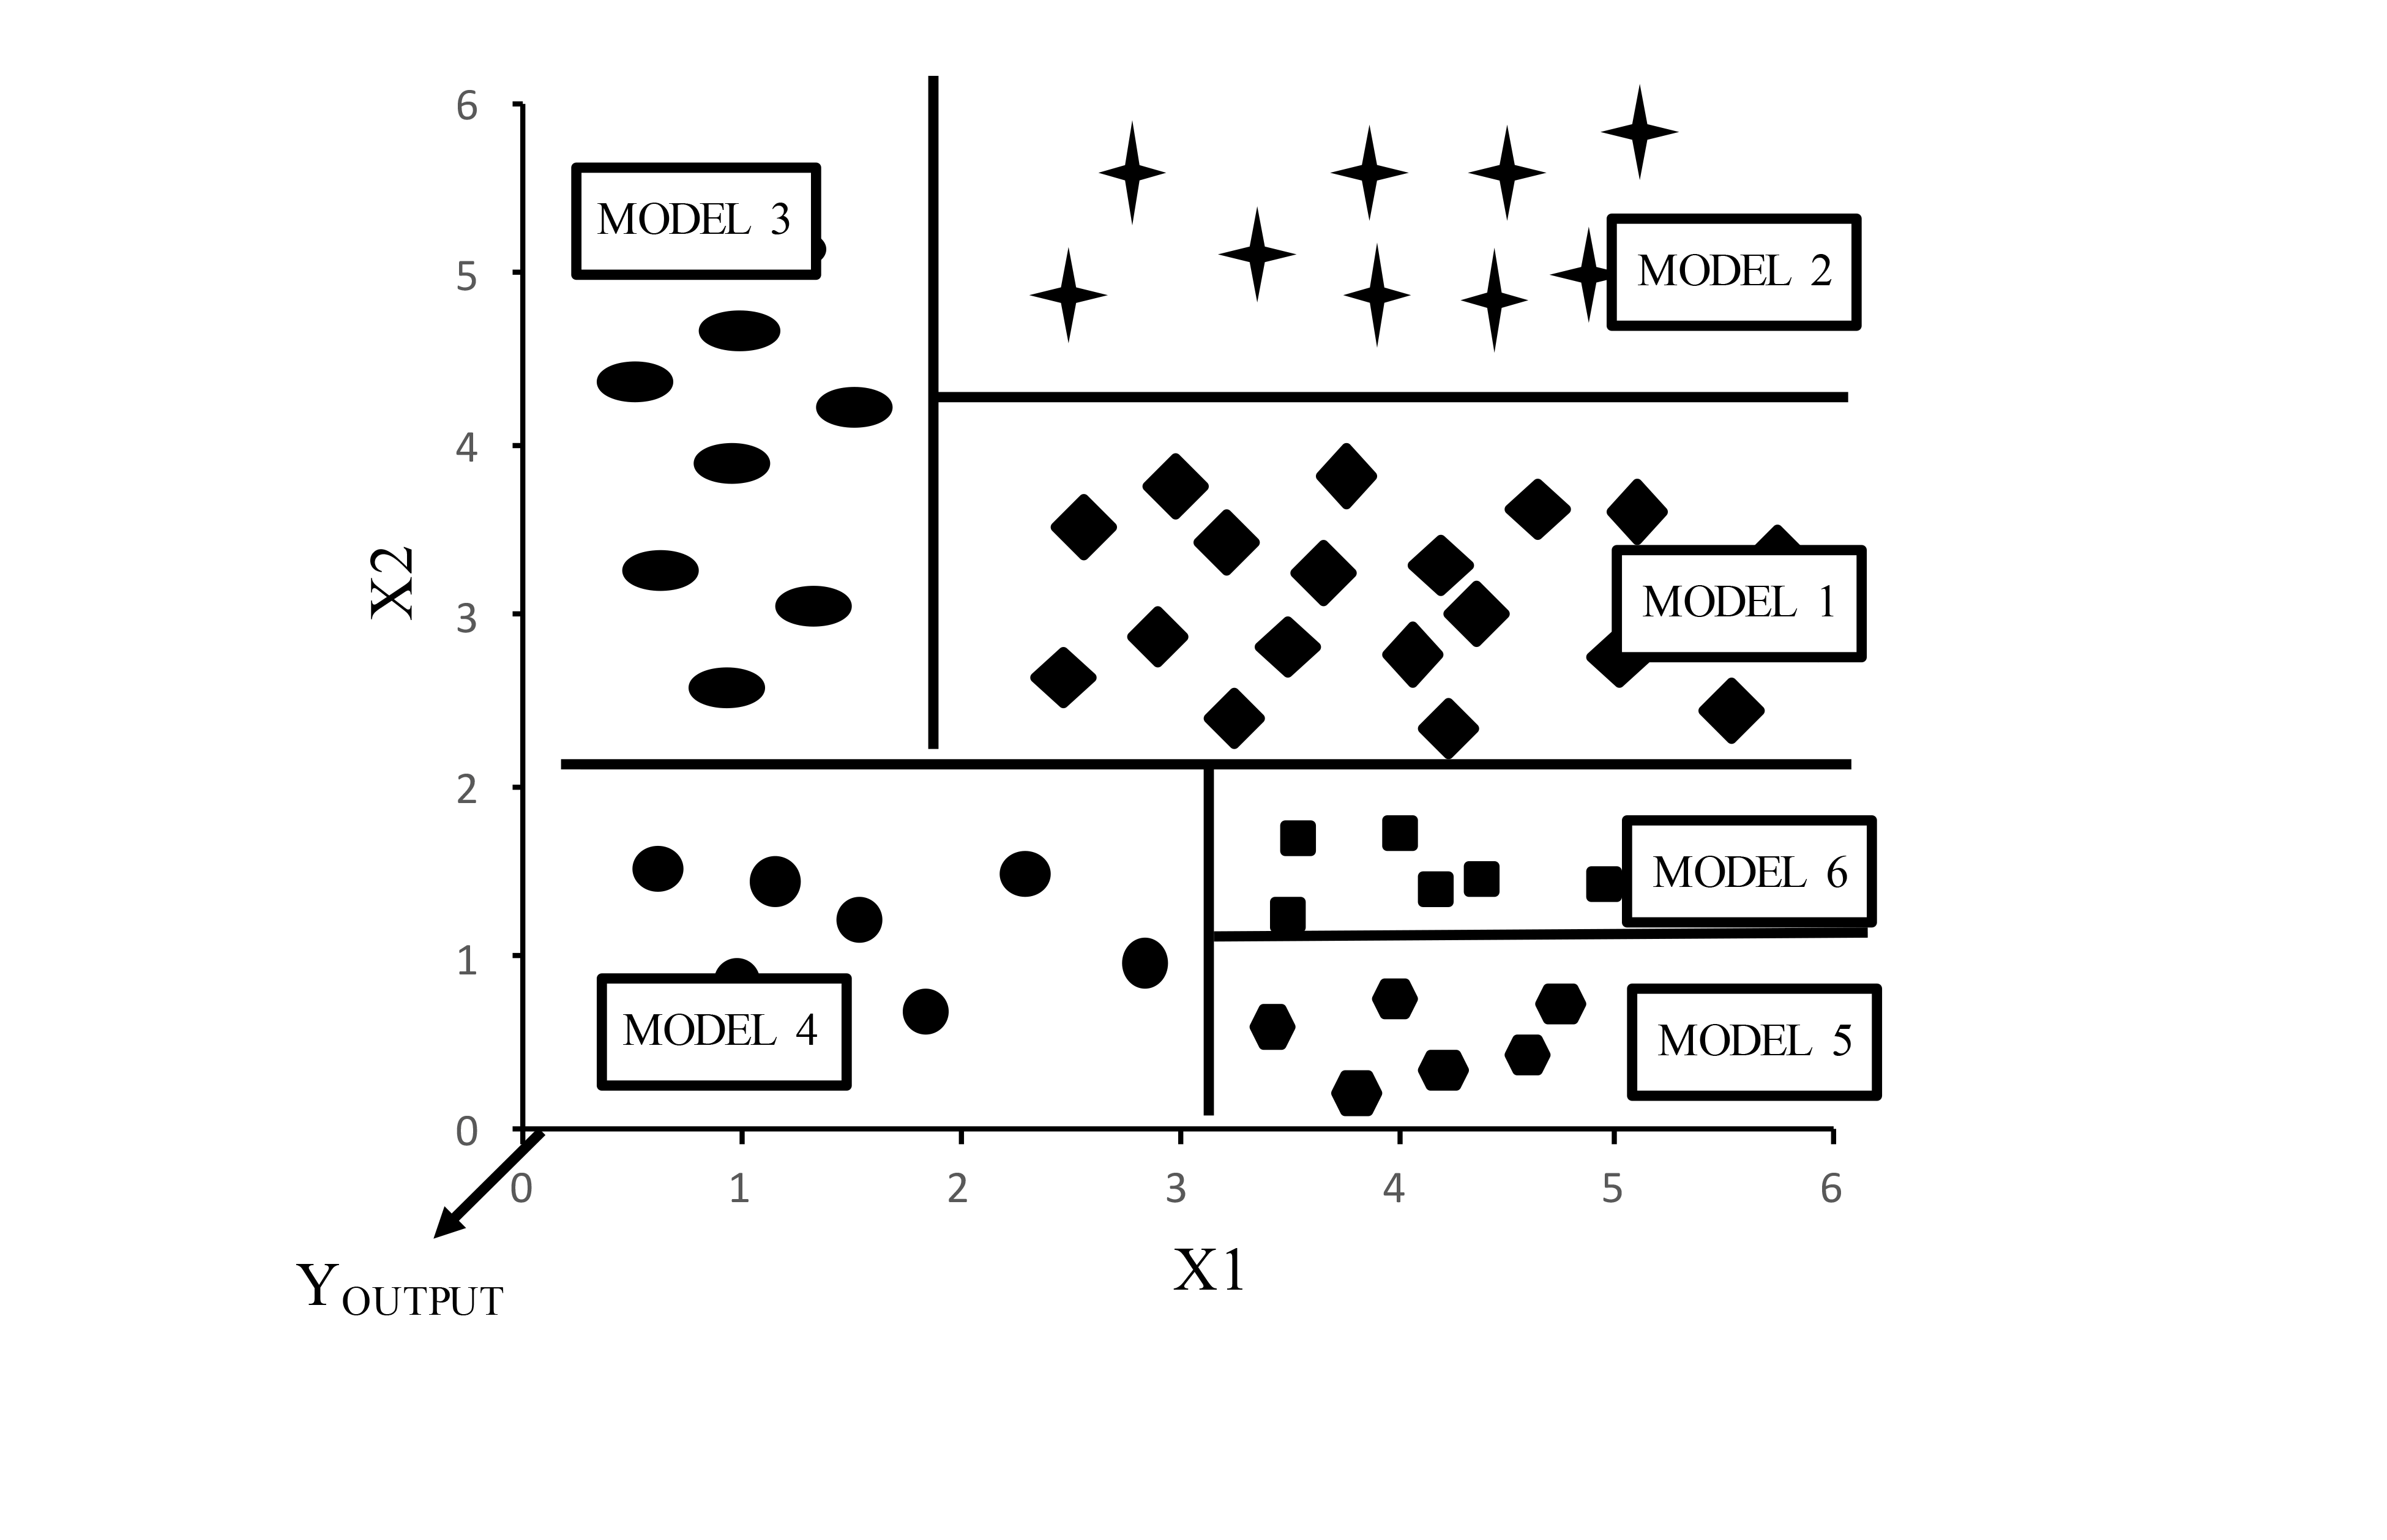
\includegraphics[height=7cm]{splits.png}
\caption{Splitting of the input space (X1 x X2) by M5' model tree algorithm}
\label{fig5}
\end{figure}

\section{Adding another section}
You can show a lot of figures together like these Figures \ref{fig61}, \ref{fig62}, \ref{fig63} below.
\begin{figure} [!htbp]
\centering    
\subfigure[Caption1]{\label{fig61}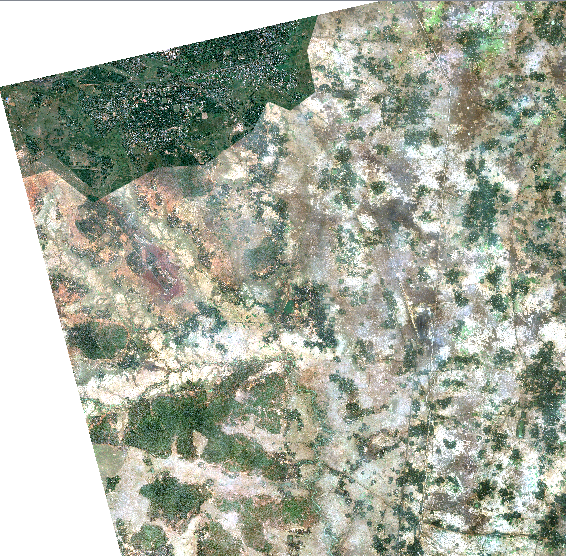
\includegraphics[width=42mm]{data1.png}}
\subfigure[Caption2]{\label{fig62}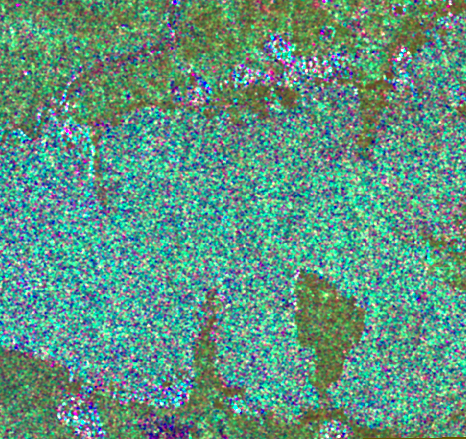
\includegraphics[width=42mm]{data2.png}}
\subfigure[Caption3]{\label{fig63}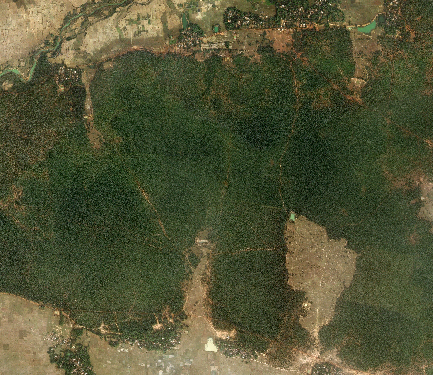
\includegraphics[width=42mm]{data3.png}}
\caption{Figures sample}
\end{figure}
You can add lists into the text like this. 
\begin{itemize}
\settowidth{\leftmargin}{{\Large$\square$}}\advance\leftmargin\labelsep
\itemsep3pt\relax
\renewcommand\labelitemi{{\lower1pt\hbox{\small$\square$}}}
\item	Some sample text item 1. 
\item You may refer to tables \ref{tab1} 
\item Or figures \ref{fig61}
\end{itemize}

Tables can be added like this
\begin{table}[!htbp]
\centering
\caption{Sample table}
\label{tab1}
\begin{tabular}{llll}

\hline
Column 1 & Column 2 & Column 3       \\\hline
1         & Data1 & 13.41179 & 0.9492839 \\
2            & Data2 & 13.39824 & 0.9492952\\\hline
\end{tabular}
\end{table}


